\documentclass{standalone}
\usepackage{tikz}
\usetikzlibrary{patterns, positioning}


\begin{document}
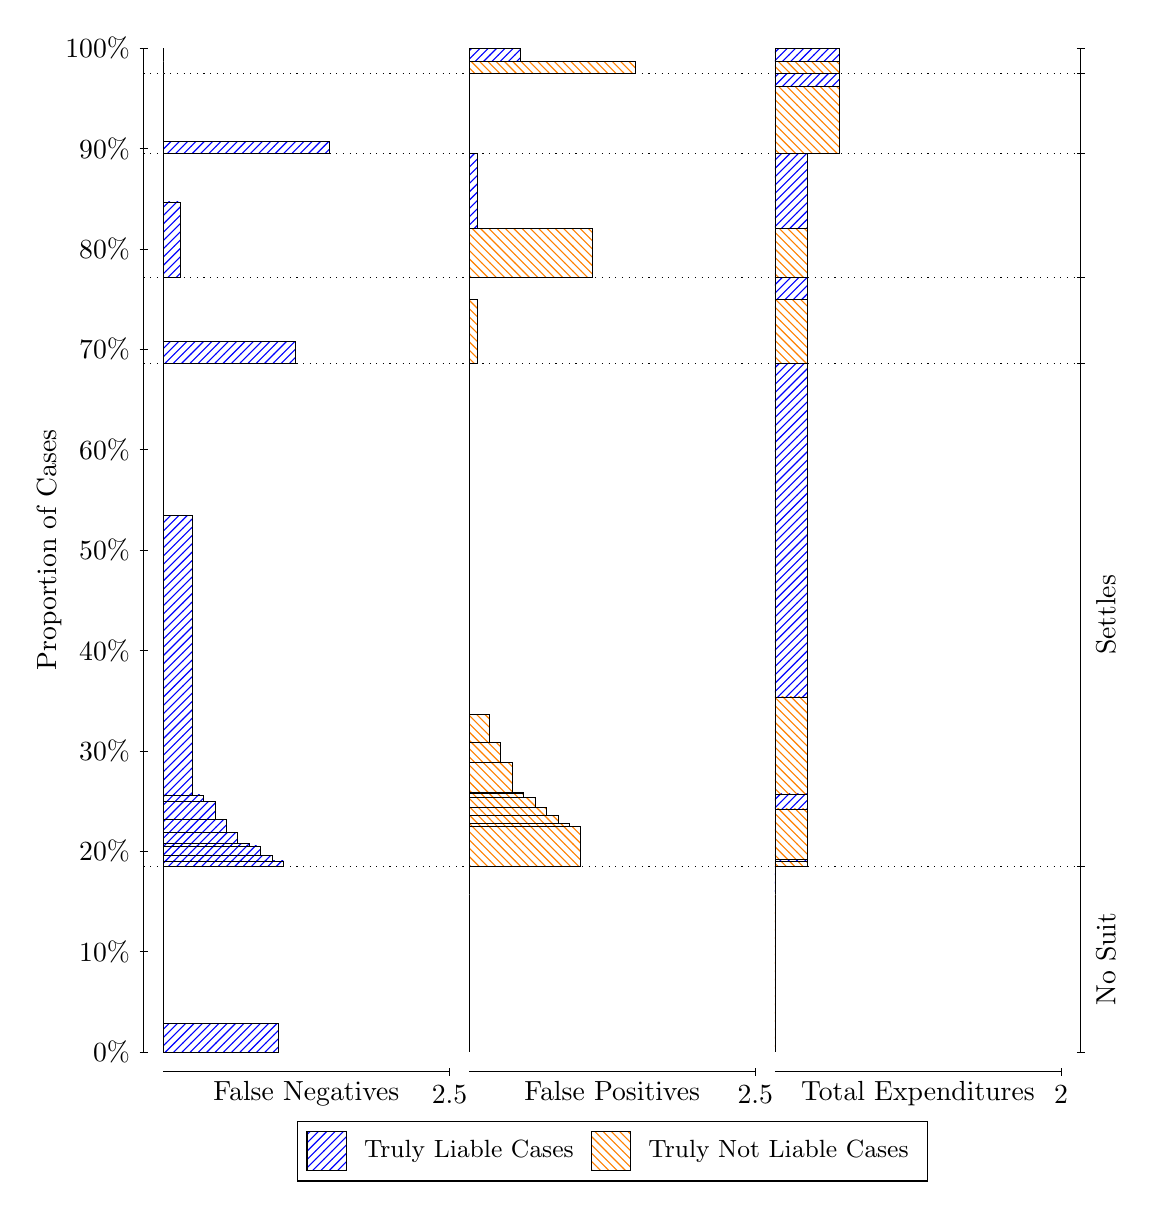
\begin{tikzpicture}
\draw[black, very thin] (1.5,1.75) -- (1.5,14.5);
\node[rotate=90, text=black, anchor=center] at (0.3, 8.125) {Proportion of Cases};
\draw[black, very thin] (1.45,1.75) -- (1.55,1.75);
\node[text=black, anchor=east] at (1.45, 1.75) {0\%};
\draw[black, very thin] (1.45,3.025) -- (1.55,3.025);
\node[text=black, anchor=east] at (1.45, 3.025) {10\%};
\draw[black, very thin] (1.45,4.3) -- (1.55,4.3);
\node[text=black, anchor=east] at (1.45, 4.3) {20\%};
\draw[black, very thin] (1.45,5.575) -- (1.55,5.575);
\node[text=black, anchor=east] at (1.45, 5.575) {30\%};
\draw[black, very thin] (1.45,6.85) -- (1.55,6.85);
\node[text=black, anchor=east] at (1.45, 6.85) {40\%};
\draw[black, very thin] (1.45,8.125) -- (1.55,8.125);
\node[text=black, anchor=east] at (1.45, 8.125) {50\%};
\draw[black, very thin] (1.45,9.4) -- (1.55,9.4);
\node[text=black, anchor=east] at (1.45, 9.4) {60\%};
\draw[black, very thin] (1.45,10.675) -- (1.55,10.675);
\node[text=black, anchor=east] at (1.45, 10.675) {70\%};
\draw[black, very thin] (1.45,11.95) -- (1.55,11.95);
\node[text=black, anchor=east] at (1.45, 11.95) {80\%};
\draw[black, very thin] (1.45,13.225) -- (1.55,13.225);
\node[text=black, anchor=east] at (1.45, 13.225) {90\%};
\draw[black, very thin] (1.45,14.5) -- (1.55,14.5);
\node[text=black, anchor=east] at (1.45, 14.5) {100\%};

\draw[black, very thin] (13.4,1.75) -- (13.4,14.5);
\draw[black, very thin] (13.35,1.75) -- (13.45,1.75);
\node[anchor=west] at (13.35, 1.75) {};
\draw[black, very thin] (13.35,4.1094) -- (13.45,4.1094);
\node[anchor=west] at (13.35, 4.1094) {};
\draw[black, very thin] (13.35,10.493) -- (13.45,10.493);
\node[anchor=west] at (13.35, 10.493) {};
\draw[black, very thin] (13.35,11.591) -- (13.45,11.591);
\node[anchor=west] at (13.35, 11.591) {};
\draw[black, very thin] (13.35,13.159) -- (13.45,13.159);
\node[anchor=west] at (13.35, 13.159) {};
\draw[black, very thin] (13.35,14.175) -- (13.45,14.175);
\node[anchor=west] at (13.35, 14.175) {};
\draw[black, very thin] (13.35,14.5) -- (13.45,14.5);
\node[anchor=west] at (13.35, 14.5) {};

\draw[black, very thin, pattern color=blue, pattern=north east lines] (1.75,1.75) rectangle (3.2033,2.1115);
\draw[black, very thin, pattern color=orange, pattern=north west lines] (1.75,2.1115) rectangle (1.75,4.1094);
\draw[black, very thin, pattern color=blue, pattern=north east lines] (1.75,4.1094) rectangle (3.276,4.1778);
\draw[black, very thin, pattern color=blue, pattern=north east lines] (1.75,4.1778) rectangle (3.1307,4.2499);
\draw[black, very thin, pattern color=blue, pattern=north east lines] (1.75,4.2499) rectangle (2.9853,4.3674);
\draw[black, very thin, pattern color=blue, pattern=north east lines] (1.75,4.3674) rectangle (2.84,4.3966);
\draw[black, very thin, pattern color=blue, pattern=north east lines] (1.75,4.3966) rectangle (2.6947,4.5429);
\draw[black, very thin, pattern color=blue, pattern=north east lines] (1.75,4.5429) rectangle (2.5493,4.7006);
\draw[black, very thin, pattern color=blue, pattern=north east lines] (1.75,4.7006) rectangle (2.404,4.9302);
\draw[black, very thin, pattern color=blue, pattern=north east lines] (1.75,4.9302) rectangle (2.2587,5.0155);
\draw[black, very thin, pattern color=blue, pattern=north east lines] (1.75,5.0155) rectangle (2.1133,8.5616);
\draw[black, very thin, pattern color=orange, pattern=north west lines] (1.75,8.5616) rectangle (1.75,10.493);
\draw[black, very thin, pattern color=blue, pattern=north east lines] (1.75,10.493) rectangle (3.4213,10.771);
\draw[black, very thin, pattern color=orange, pattern=north west lines] (1.75,10.771) rectangle (1.75,11.591);
\draw[black, very thin, pattern color=blue, pattern=north east lines] (1.75,11.591) rectangle (1.968,12.545);
\draw[black, very thin, pattern color=orange, pattern=north west lines] (1.75,12.545) rectangle (1.75,13.159);
\draw[black, very thin, pattern color=blue, pattern=north east lines] (1.75,13.159) rectangle (3.8573,13.319);
\draw[black, very thin, pattern color=orange, pattern=north west lines] (1.75,13.319) rectangle (1.75,14.175);
\draw[black, very thin, pattern color=orange, pattern=north west lines] (1.75,14.175) rectangle (1.75,14.331);
\draw[black, very thin, pattern color=blue, pattern=north east lines] (1.75,14.331) rectangle (1.75,14.5);
\draw[black, very thin, pattern color=orange, pattern=north west lines] (5.6333,1.75) rectangle (5.6333,3.7478);
\draw[black, very thin, pattern color=blue, pattern=north east lines] (5.6333,3.7478) rectangle (5.6333,4.1094);
\draw[black, very thin, pattern color=orange, pattern=north west lines] (5.6333,4.1094) rectangle (7.0503,4.6144);
\draw[black, very thin, pattern color=orange, pattern=north west lines] (5.6333,4.6144) rectangle (6.905,4.6566);
\draw[black, very thin, pattern color=orange, pattern=north west lines] (5.6333,4.6566) rectangle (6.7597,4.7542);
\draw[black, very thin, pattern color=orange, pattern=north west lines] (5.6333,4.7542) rectangle (6.6143,4.856);
\draw[black, very thin, pattern color=orange, pattern=north west lines] (5.6333,4.856) rectangle (6.469,4.9785);
\draw[black, very thin, pattern color=orange, pattern=north west lines] (5.6333,4.9785) rectangle (6.3237,5.036);
\draw[black, very thin, pattern color=orange, pattern=north west lines] (5.6333,5.036) rectangle (6.3237,5.0425);
\draw[black, very thin, pattern color=orange, pattern=north west lines] (5.6333,5.0425) rectangle (6.1783,5.4302);
\draw[black, very thin, pattern color=orange, pattern=north west lines] (5.6333,5.4302) rectangle (6.033,5.6775);
\draw[black, very thin, pattern color=orange, pattern=north west lines] (5.6333,5.6775) rectangle (5.8877,6.0409);
\draw[black, very thin, pattern color=blue, pattern=north east lines] (5.6333,6.0409) rectangle (5.6333,10.493);
\draw[black, very thin, pattern color=orange, pattern=north west lines] (5.6333,10.493) rectangle (5.7423,11.312);
\draw[black, very thin, pattern color=blue, pattern=north east lines] (5.6333,11.312) rectangle (5.6333,11.591);
\draw[black, very thin, pattern color=orange, pattern=north west lines] (5.6333,11.591) rectangle (7.1957,12.205);
\draw[black, very thin, pattern color=blue, pattern=north east lines] (5.6333,12.205) rectangle (5.7423,13.159);
\draw[black, very thin, pattern color=orange, pattern=north west lines] (5.6333,13.159) rectangle (5.6333,14.015);
\draw[black, very thin, pattern color=blue, pattern=north east lines] (5.6333,14.015) rectangle (5.6333,14.175);
\draw[black, very thin, pattern color=orange, pattern=north west lines] (5.6333,14.175) rectangle (7.7407,14.331);
\draw[black, very thin, pattern color=blue, pattern=north east lines] (5.6333,14.331) rectangle (6.2873,14.5);
\draw[black, very thin, pattern color=orange, pattern=north west lines] (9.5167,1.75) rectangle (9.5167,3.7478);
\draw[black, very thin, pattern color=blue, pattern=north east lines] (9.5167,3.7478) rectangle (9.5167,4.1094);
\draw[black, very thin, pattern color=orange, pattern=north west lines] (9.5167,4.1094) rectangle (9.9254,4.1669);
\draw[black, very thin, pattern color=blue, pattern=north east lines] (9.5167,4.1669) rectangle (9.9254,4.1947);
\draw[black, very thin, pattern color=orange, pattern=north west lines] (9.5167,4.1947) rectangle (9.9254,4.8362);
\draw[black, very thin, pattern color=blue, pattern=north east lines] (9.5167,4.8362) rectangle (9.9254,5.0272);
\draw[black, very thin, pattern color=orange, pattern=north west lines] (9.5167,5.0272) rectangle (9.9254,6.2596);
\draw[black, very thin, pattern color=blue, pattern=north east lines] (9.5167,6.2596) rectangle (9.9254,10.493);
\draw[black, very thin, pattern color=orange, pattern=north west lines] (9.5167,10.493) rectangle (9.9254,11.312);
\draw[black, very thin, pattern color=blue, pattern=north east lines] (9.5167,11.312) rectangle (9.9254,11.591);
\draw[black, very thin, pattern color=orange, pattern=north west lines] (9.5167,11.591) rectangle (9.9254,12.205);
\draw[black, very thin, pattern color=blue, pattern=north east lines] (9.5167,12.205) rectangle (9.9254,13.159);
\draw[black, very thin, pattern color=orange, pattern=north west lines] (9.5167,13.159) rectangle (10.334,14.015);
\draw[black, very thin, pattern color=blue, pattern=north east lines] (9.5167,14.015) rectangle (10.334,14.175);
\draw[black, very thin, pattern color=orange, pattern=north west lines] (9.5167,14.175) rectangle (10.334,14.331);
\draw[black, very thin, pattern color=blue, pattern=north east lines] (9.5167,14.331) rectangle (10.334,14.5);
\draw[black, dotted] (1.5,4.1094) -- (13.4,4.1094);
\draw[black, dotted] (1.5,10.493) -- (13.4,10.493);
\draw[black, dotted] (1.5,11.591) -- (13.4,11.591);
\draw[black, dotted] (1.5,13.159) -- (13.4,13.159);
\draw[black, dotted] (1.5,14.175) -- (13.4,14.175);
\draw[black, very thin] (1.75,1.5) -- (5.3833,1.5);
\node[text=black, anchor=north] at (3.5667, 1.5) {False Negatives};
\draw[black, very thin] (5.3833,1.45) -- (5.3833,1.55);
\node[text=black, anchor=north] at (5.3833, 1.45) {2.5};

\draw[black, very thin] (5.6333,1.5) -- (9.2667,1.5);
\node[text=black, anchor=north] at (7.45, 1.5) {False Positives};
\draw[black, very thin] (9.2667,1.45) -- (9.2667,1.55);
\node[text=black, anchor=north] at (9.2667, 1.45) {2.5};

\draw[black, very thin] (9.5167,1.5) -- (13.15,1.5);
\node[text=black, anchor=north] at (11.333, 1.5) {Total Expenditures};
\draw[black, very thin] (13.15,1.45) -- (13.15,1.55);
\node[text=black, anchor=north] at (13.15, 1.45) {2};

\node[text=black, centered, rotate=90] at (13.72, 2.9297) {No Suit};
\node[text=black, centered, rotate=90] at (13.72, 7.3012) {Settles};





\draw (7.449999999999999,1.5) node[draw=none] (baseCoordinate) {};
\begin{scope}[align=center]
        \matrix[scale=0.5, draw=black, below=0.5cm of baseCoordinate, nodes={draw}, column sep=0.1cm]{
            \node[rectangle, draw, minimum width=0.5cm, minimum height=0.5cm, pattern color=blue, pattern=north east lines] {}; &
            \node[draw=none, font=\small, text=black] (B) {Truly Liable Cases}; &
            \node[rectangle, draw, minimum width=0.5cm, minimum height=0.5cm, pattern color=orange, pattern=north west lines] {}; &
            \node[draw=none, font=\small, text=black] (B) {Truly Not Liable Cases}; \\
            };
\end{scope}

\end{tikzpicture}
\end{document}